\section{TEORÍA}
\subsection{Máquinas de Estados Finitos}
\begin{frame}{TEORÍA}
\framesubtitle{Máquinas de Estados Finitos}
    Modelo computacional para simular lógica secuencial, utilizando hardware o software\footnote{\bibentry{brilliantFinite}}. Éstas son utilizadas en:
        \begin{itemize}
            \item Matemáticas
            \item Inteligencia Artificial
            \item Juegos
            \item Lingüística
        \end{itemize}
        Y están completamente descritas por una tupla de 5 elementos:
        \begin{multicols}{2}
          \begin{equation*}
          	(Q,\Sigma,\delta,q_0,F)
          \end{equation*}
          \columnbreak
          \begin{itemize}
          \item $Q=$ conjunto finito de estados
          \item $\Sigma=$ alfabeto finito y no vacío
          \item $\delta=$ funciones de transición
          \item $q_0=$ estado inicial
          \item $F=$ conjunto de estados que acepta
          \end{itemize}\end{multicols}
\end{frame}

\begin{frame}{TEORÍA}
    \framesubtitle{Máquinas de Estados Finitos}
    \begin{figure}[H]
        \centering
        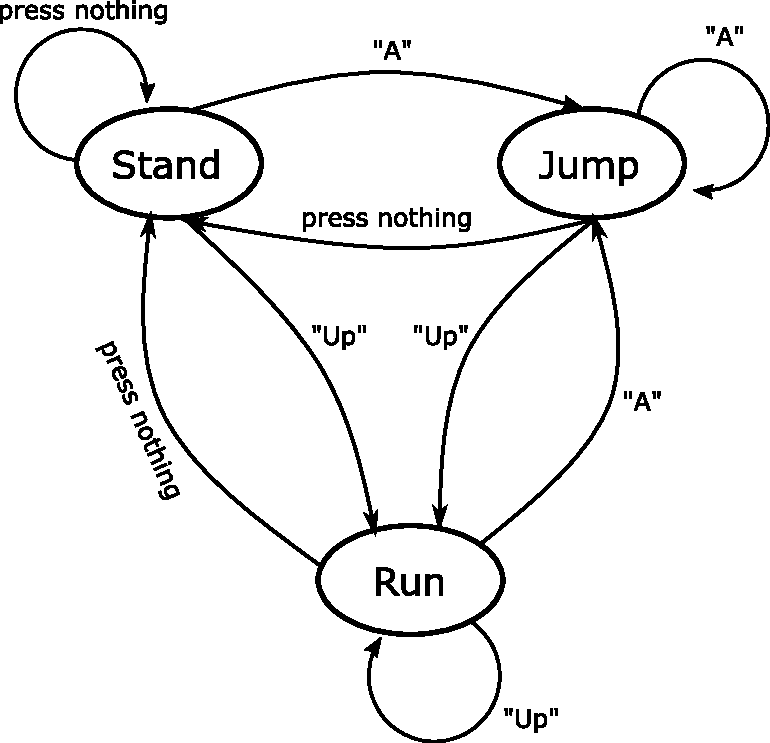
\includegraphics[scale=0.3]{files/Finite.pdf}
        \caption{Máquina de estados finitos para un personaje en video juego simple\footnotemark{}.}
    \end{figure}
    \footnotetext{\bibentry{brilliantFinite}}
    \begin{itemize}
        \item Son poco eficientes para programar
        \item No imitan correctamente el comportamiento humano
        \item Se debe utilizar una distinta para cada problema
    \end{itemize}
\end{frame}

\subsection{Cadenas de Markov}
\begin{frame}{TEORÍA}
    \framesubtitle{Cadenas de Markov}
    Es una representación matemática de un sistema que puede pasar de un estado a otro de acuerdo a unas probabilidades definidas a estas transiciones.
    \begin{figure}[H]
        \centering
        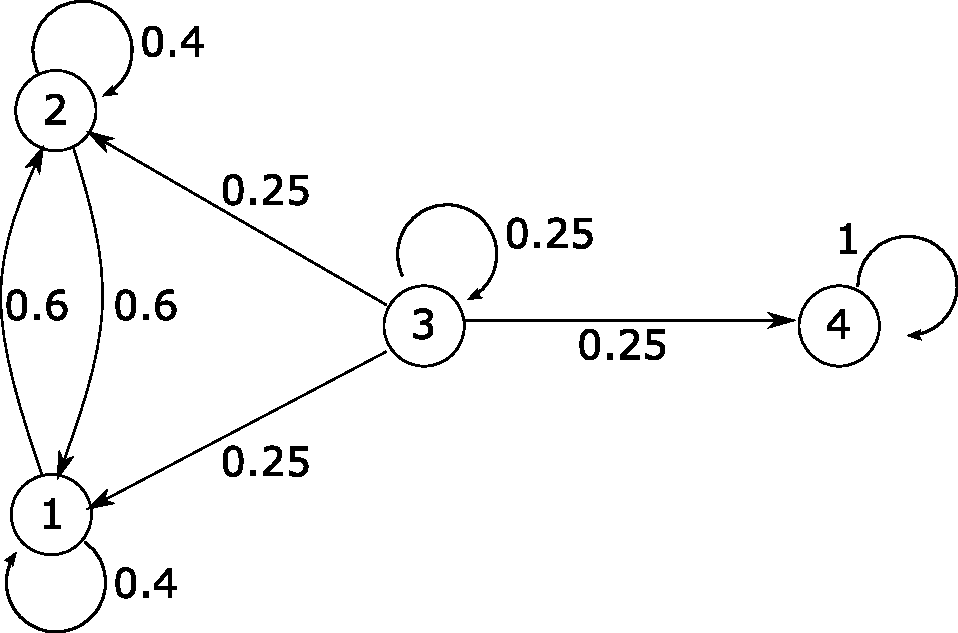
\includegraphics[scale=0.3]{files/Markov.pdf}
        \caption{Ejemplo Cadena de Markov con 4 estados\footnotemark{}.}
    \end{figure}
    \footnotetext{\bibentry{brilliantMarkov}}
\end{frame}

\begin{frame}{TEORÍA}
    \framesubtitle{Cadenas de Markov}
    Deben cumplir la propiedad de Markov\footnote{\bibentry{brilliantMarkov}}:
    \begin{center}
        \textit{``La probabilidad de las acciones futuras no dependen de los pasos que llevaron al estado actual''}
    \end{center}
    \textbf{Definición formal}

    Sea $S=\{i_1$, $i_2$, $...$, $i_n\}$ el conjunto de los posibles estados del sistema, una Cadena de Markov puede definirse como una secuencia de variables aleatorias $X_1$, $X_2$, $X_3$, $...$ tales que $\forall n\in \mathbb{Z^+}$ y $\forall i_k\in S$
    \begin{equation}
        P(X_n = i_n \mid X_0 = i_0, \, X_1 = i_1, \, \dots, \, X_{n-1} = i_{n-1}) = P(X_n = i_n \mid X_{n-1} = i_{n-1})
    \end{equation}
\end{frame}



\subsection{Análisis Bayesiano}
\begin{frame}{TEORÍA}
    \framesubtitle{Análisis Bayesiano}
    \textbf{Definición}

    El análisis bayesiano hace parte de las dos escuelas para hacer análisis estadístico: frecuencialista y bayesiana. El análisis bayesiano se puede definir como:
    \begin{center}
        \textit{``Conjunto de métodos prácticos para hacer inferencias de datos utilizando modelos de probabilidad para cantidades que observamos y de las que queremos aprender'' \footnote{\bibentry{gelman2013bayesian}}.}
    \end{center}
\end{frame}

\begin{frame}{TEORÍA}
    \framesubtitle{Análisis Bayesiano}
    Sea $y$ un conjunto de datos conocido y $\theta$ los parámetros que generaron estos datos.

    \begin{multicols}{2}
        \textbf{Enfoque Frecuencialista}

        \begin{itemize}
            \item Los datos analizados son producto de un proceso aleatorio, los datos cambiarán cada vez que sean recolectados.
            \item Se analizan probabildades de la forma
            \begin{equation*}
                P(y\mid\theta)
            \end{equation*}
            \item Se crean estimadores para asignar valores a $\theta$, son diferentes para cada problema.
        \end{itemize}\columnbreak
        \textbf{Enfoque Bayesiano}

        \begin{itemize}
            \item Los datos no son aleatorios una vez son recolectados.
            \item Se analizan probabilidades de la forma
            \begin{equation*}
                P(\theta\mid y)
            \end{equation*}
            \item Se utiliza un único estimador: fórmula de Bayes.
            \item $\theta$ y $y$ son fijados, pero el conocimiento acerca de los valores de $\theta$ cambia\footnote{\bibentry{youtube1}}.
        \end{itemize}
    \end{multicols}
\end{frame}

\begin{frame}{TEORÍA}
    \framesubtitle{Análisis Bayesiano}
    \textbf{Contrucción del modelo bayesiano\footnote{\bibentry{gelman2013bayesian}}}

    \begin{enumerate}
        \item \textit{Especificar un modelo de probabilidad}: Que incluya todas variables influyentes y de las cuales se espera aprender
        \item \textit{Calcular la distribución a posteriori}: Nos proporciona información acerca del $\theta$ desconocido después de haber observado $y$. Su dificultad promueve el enfoque frecuencialista.
        \item \textit{Validar el modelo}: Como el modelo está ligado a todas las predicciones e inferencias, éste debe ser revisado
    \end{enumerate}
\end{frame}

\begin{frame}{TEORÍA}
    \framesubtitle{Fórmula de Bayes\footnote{\bibentry{youtube1}}}
    \begin{equation}
        P(\theta\mid y)=\frac{P(y\mid\theta)P(\theta)}{P(y)}
    \end{equation}
    Donde
    \begin{itemize}
        \item $P(\theta\mid y)$ es la distribución a posteriori
        \item $P(\theta)$ es la distribución a priori
        \item $P(y\mid\theta)$ es la verosimilitud
        \item $P(y)$ es el factor de normalización
    \end{itemize}
\end{frame}
